\documentclass{standalone}
\usepackage{tikz}
\usepackage{amssymb}
\usetikzlibrary{positioning, shapes, arrows,}

\begin{document}
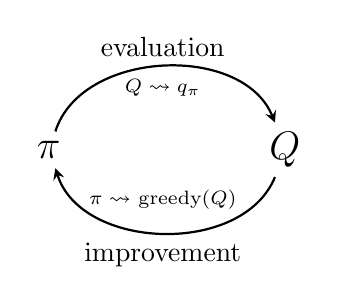
\begin{tikzpicture}[>=stealth, node distance=1.5cm, on grid, auto,
    arrow/.style = {thick,-stealth}]

    % States
    \node [] (center) {};
    \node [] (policy) [left=of center ] {\Large \(\pi\)};
    \node [] (values) [right=of center] {\Large \(Q\)};

    % Transitions
    \draw [arrow] (policy) edge[bend left=70] node(E) {evaluation} (values);
    \draw [arrow] (values) edge[bend left=70] node(I) {improvement} (policy);
    \node [] () [below= 15pt of E] {\scriptsize\(Q\rightsquigarrow q_\pi\)};
    \node [] () [above= 20pt of I] {\scriptsize\(\pi\rightsquigarrow\) greedy\((Q)\)};
\end{tikzpicture}


\end{document}